\documentclass[a4paper, 11pt]{article}
\usepackage[hmargin=1in]{geometry}
\usepackage[utf8]{inputenc}
\usepackage[T1, T2A]{fontenc}
\usepackage{csquotes}
\usepackage[main=bulgarian, english]{babel}
\usepackage{amsmath}
\usepackage{amssymb}
\usepackage{amsthm}
\usepackage{listings}
\usepackage{graphicx}
\usepackage{float}
\usepackage{svg}
\usepackage{tikz}
\usepackage{helvet}
\usepackage{xcolor}
\usepackage[style=numeric, sorting=none, language=auto]{biblatex}
\usepackage[hidelinks]{hyperref}
\addbibresource{sources.bib}
\allowdisplaybreaks

\begin{document}
\author{Даниел Халачев, ИИОЗ, 4MI3400603}
\title{Онтология на основните стилове в изобразителното изкуство и техните отличителни картини}
\maketitle

\pagebreak
\tableofcontents
\pagebreak
\section{Въведение}
Главната цел на проекта е да се създаде структурата на онтология, която представя основните епохи от човешкото развитие, типичните за тях стилове от изобразителното изкуство и връзките между тях, и знакови картини от дадени стилове. Онтологията съдържа:
\begin{itemize}
  \item 17 концепта
  \item 12 роли
  \item 71 константи.
\end{itemize}
\section{Структура}
\subsection{Атомарни концепти}
\begin{itemize}
  \item \textbf{Artwork} - произведение на изкуството
  \item \textbf{Age} - епоха в човешкото развитие
  \item \textbf{Style} - стил в изобразителното изкуство
  \item \textbf{Artist} - художник, нарисувал картината
  \item \textbf{Region} - регион на света, където е работил художникът
  \item \textbf{Medium} - средство за изобразяване
  \item \textbf{Depiction} - какво изобразява картината
  \item \textbf{Museum} - музей, в който се помещава картината днес
\end{itemize}
\subsection{Атомарни подконцепти}
\begin{align*}
  &\text{Paint} \sqsubseteq \text{Medium} \\
  &\text{Landscape} \sqsubseteq \text{Depiction}
\end{align*}

\subsection{Неатомарни концепти}
\begin{align*}
  \text{Painting} &\doteq \text{[AND Artwork [EXISTS 1 :depicts] [EXISTS 1 :hasMedium]]} \\
  \text{OilPainting} &\doteq \text{[AND Painting [FILLS :hasMedium OilPaint]]} \\
  \text{AcrylicPainting} &\doteq \text{[AND Painting [FILLS :hasMedium AcrylicPaint]]} \\
  \text{PortraitPainting} &\doteq \text{[AND Painting [FILLS :depicts Portrait]]} \\
  \text{LandscapePainting} &\doteq \text{[AND Painting [ALL :depicts Landscape]]} \\
  \text{PortraitOilPainting} &\doteq \text{[AND OilPainting PortraitPainting]} \\
  \text{HistoricalEventOilPainting} &\doteq \text{[AND OilPainting [FILLS :depicts HistoricalEvent]]} \\
\end{align*}

\subsection{Роли}
\begin{align*}
  \text{belongsTo} &: \text{Style} \to \text{Age}\\
  \text{represents} &: \text{Artwork} \to \text{Style}\\
  \text{createdBy} &: \text{Artwork} \to \text{Artist}\\
  \text{housedIn} &: \text{Artwork} \to \text{Museum}\\
  \text{locatedIn} &: \text{Museum} \to \text{Region}\\
  \text{negativeReactionTo} &: \text{Style} \to \text{Style}\\
  \text{positiveReactionTo} &: \text{Style} \to \text{Style}\\
  \text{depicts} &: \text{Painting} \to \text{Depiction}\\
  \text{usesMedium} &: \text{Painting} \to \text{Medium}\\
  \text{livedIn} &: \text{Artist} \to \text{Region}\\
  \text{precededBy} &: \text{Age} \to \text{Age}\\
  \text{succeededBy} &: \text{Age} \to \text{Age}.
\end{align*}
От тях \emph{precededBy} и \emph{succeededBy} са противоположни и транзитивни, а \emph{createdBy} и \emph{housedIn} са функционални.

\section{Константи}
\subsection{Age (8)}
    \begin{align*}
      \text{PrehistoricAge} \to& \text{Age}\\
      \text{Antiquity} \to& \text{[AND}\\
      &\quad\text{Age}\\
      &\quad\text{[FILLS :succeededBy MiddleAges]]}\\\\
      \text{MiddleAges} \to& \text{[AND}\\
      &\quad\text{Age}\\
      &\quad\text{[FILLS :precededBy Antiquity]}\\
      &\quad\text{[FILLS :succeededBy Renaissance]]}\\\\  
      \text{GothicAge} \to& \text{[AND}\\
      &\quad\text{Age}\\
      &\quad\text{[FILLS :precededBy MiddleAges]}\\
      &\quad\text{[FILLS :succeededBy Renaissance]]}\\\\
      \text{Renaissance} \to& \text{[AND}\\
      &\quad\text{Age}\\
      &\quad\text{[FILLS :precededBy MiddleAges]}\\
      &\quad\text{[FILLS :succeededBy NewAge]]}\\\\
      \text{NewAge} \to& \text{[AND}\\
      &\quad\text{Age}\\
      &\quad\text{[FILLS :precededBy Renaissance]}\\
      &\quad\text{[FILLS :succeededBy ModernAge]]}\\\\
      \text{ModernAge} \to& \text{[AND}\\
      &\quad\text{Age}\\
      &\quad\text{[FILLS :precededBy NewAge]}\\
      &\quad\text{[FILLS :succeededBy ContemporaryAge]]}\\\\
      \text{ContemporaryAge} \to& \text{[AND}\\
      &\quad\text{Age}\\
      &\quad\text{[FILLS :precededBy ModernAge]]}
    \end{align*}
    
  \subsection{Style (25)}
    \begin{align*}
      \text{Paleolithic} \to& \text{[AND}\\
      &\quad\text{Style}\\
      &\quad\text{[FILLS :belongsTo PrehistoricAge]]}\\\\
      \text{Neolithic} \to& \text{[AND}\\
      &\quad\text{Style}\\
      &\quad\text{[FILLS :belongsTo PrehistoricAge]]}\\\\
      \text{AncientEgyptian} \to& \text{[AND}\\
      &\quad\text{Style}\\
      &\quad\text{[FILLS :belongsTo Antiquity]]}\\\\
      \text{AncientGreek} \to& \text{[AND}\\
      &\quad\text{Style}\\
      &\quad\text{[FILLS :belongsTo Antiquity]}\\
      &\quad\text{[FILLS :positiveReactionTo AncientEgyptian]]}\\\\
      \text{Roman} \to& \text{[AND}\\
      &\quad\text{Style}\\
      &\quad\text{[FILLS :belongsTo Antiquity]}\\
      &\quad\text{[FILLS :positiveReactionTo AncientGreek]]}\\\\
      \text{Byzantine} \to& \text{[AND}\\
      &\quad\text{Style}\\
      &\quad\text{[FILLS :belongsTo MiddleAges]]}\\\\
      \text{Romanesque} \to& \text{[AND}\\
      &\quad\text{Style}\\
      &\quad\text{[FILLS :belongsTo MiddleAges]]}\\\\
      \text{Gothic} \to& \text{[AND}\\
      &\quad\text{Style}\\
      &\quad\text{[FILLS :belongsTo GothicAge]}\\
      &\quad\text{[FILLS :positiveReactionTo Romanesque]]}\\\\
      \text{ItalianRenaissance} \to& \text{[AND}\\
      &\quad\text{Style}\\
      &\quad\text{[FILLS :belongsTo Renaissance]}\\
      &\quad\text{[FILLS :negativeReactionTo Gothic]]}\\\\
      \text{NordicRenaissance} \to& \text{[AND}\\
      &\quad\text{Style}\\
      &\quad\text{[FILLS :belongsTo Renaissance]]}\\\\
      \text{Baroque} \to& \text{[AND}\\
      &\quad\text{Style}\\
      &\quad\text{[FILLS :belongsTo NewAge]}\\
      &\quad\text{[FILLS :negativeReactionTo Renaissance]]}\\\\
      \text{Rococo} \to& \text{[AND}\\
      &\quad\text{Style}\\
      &\quad\text{[FILLS :belongsTo NewAge]}\\
      &\quad\text{[FILLS :negativeReactionTo Baroque]]}\\\\
      \text{Classicism} \to& \text{[AND}\\
      &\quad\text{Style}\\
      &\quad\text{[FILLS :belongsTo NewAge]}\\
      &\quad\text{[FILLS :negativeReactionTo Rococo]]}\\\\
      \text{Romanticism} \to& \text{[AND}\\
      &\quad\text{Style}\\
      &\quad\text{[FILLS :belongsTo NewAge]]}\\\\
      \text{Realism} \to& \text{[AND}\\
      &\quad\text{Style}\\
      &\quad\text{[FILLS :belongsTo ModernAge]}\\
      &\quad\text{[FILLS :negativeReactionTo Romanticism]]}\\\\
      \text{Impressionism} \to& \text{[AND}\\
      &\quad\text{Style}\\
      &\quad\text{[FILLS :belongsTo ModernAge]}\\
      &\quad\text{[FILLS :negativeReactionTo Realism]]}\\\\
      \text{PostImpressionism} \to& \text{[AND}\\
      &\quad\text{Style}\\
      &\quad\text{[FILLS :belongsTo ModernAge]}\\
      &\quad\text{[FILLS :positiveReactionTo Impressionism]]}\\\\
      \text{Expressionism} \to& \text{[AND}\\
      &\quad\text{Style}\\
      &\quad\text{[FILLS :belongsTo ModernAge]}\\
      &\quad\text{[FILLS :negativeReactionTo Realism]]}\\\\
      \text{Cubism} \to& \text{[AND}\\
      &\quad\text{Style}\\
      &\quad\text{[FILLS :belongsTo ModernAge]}\\
      &\quad\text{[FILLS :negativeReactionTo Impressionism]]}\\\\
      \text{Futurism} \to& \text{[AND}\\
      &\quad\text{Style}\\
      &\quad\text{[FILLS :belongsTo ModernAge]]}\\\\
      \text{Dadaism} \to& \text{[AND}\\
      &\quad\text{Style}\\
      &\quad\text{[FILLS :belongsTo ModernAge]]}\\\\
      \text{Surrealism} \to& \text{[AND}\\
      &\quad\text{Style}\\
      &\quad\text{[FILLS :belongsTo ModernAge]}\\
      &\quad\text{[FILLS :positiveReactionTo Dadaism]]}\\\\
      \text{PopArt} \to& \text{[AND}\\
      &\quad\text{Style}\\
      &\quad\text{[FILLS :belongsTo ContemporaryAge]]}\\\\
      \text{ConceptualArt} \to& \text{[AND}\\
      &\quad\text{Style}\\
      &\quad\text{[FILLS :belongsTo ContemporaryAge]}\\
      &\quad\text{[FILLS :positiveReactionTo PopArt]]}
    \end{align*}
    \subsection{Region (7)}
        \begin{align*}
        \text{Asia} &\to \text{Region}\\
        \text{Africa} &\to \text{Region}\\
        \text{Australia} &\to \text{Region}\\
        \text{SouthAmerica} &\to \text{Region}\\
        \text{NorthAmerica} &\to \text{Region}\\
        \text{EasternEurope} &\to \text{Region}\\
        \text{WesternEurope} &\to \text{Region}
        \end{align*}
    \subsection{Medium (4)}
        \begin{align*}
        \text{Chalk} &\to \text{Medium}\\
        \text{Graphite} &\to \text{Medium}\\
        \text{OilPaint} &\to \text{Paint} \sqsubseteq \text{Medium}\\
        \text{AcrylicPaint} &\to \text{Paint} \sqsubseteq \text{Medium}
        \end{align*}
    \subsection{Depiction (6)}
        \begin{align*}
        \text{AbstractDepiction} &\to \text{Depiction}\\
        \text{GroupScene} &\to \text{Depiction}\\
        \text{Portrait} &\to \text{Depiction}\\
        \text{HistoricalEvent} &\to \text{Depiction}\\
        \text{UrbanLandscape} &\to \text{Landscape}\sqsubseteq \text{Depiction}\\
        \text{NaturalLandscape} &\to \text{Landscape}\sqsubseteq \text{Depiction}\\
        \end{align*}
    \subsection{Artist (7)}
    \begin{align*}
    \text{Michelangelo} \to& \text{[AND} \\
    &\quad \text{Artist} \\
    &\quad \text{[FILLS :livedIn WesternEurope]]} \\
    \text{VincentVanGogh} \to& \text{[AND} \\
    &\quad \text{Artist} \\
    &\quad \text{[FILLS :livedIn WesternEurope]]} \\
    \text{JohannesVermeer} \to& \text{[AND} \\
    &\quad \text{Artist} \\
    &\quad \text{[FILLS :livedIn WesternEurope]]} \\
    \text{LeonardoDaVinci} \to& \text{[AND} \\
    &\quad \text{Artist} \\
    &\quad \text{[FILLS :livedIn WesternEurope]]} \\
    \text{FranciscoGoya} \to& \text{[AND} \\
    &\quad \text{Artist} \\
    &\quad \text{[FILLS :livedIn WesternEurope]]} \\
    \text{AndyWarhol} \to& \text{[AND} \\
    &\quad \text{Artist} \\
    &\quad \text{[FILLS :livedIn NorthAmerica]]} \\
    \text{ClaudeMonet} \to& \text{[AND} \\
    &\quad \text{Artist} \\
    &\quad \text{[FILLS :livedIn WesternEurope]]}
    \end{align*}
    
    \subsection{Museum (7)}
    \begin{align*}
    \text{GalleriaDellAccademia} \to& \text{[AND} \\
    &\quad \text{Museum} \\
    &\quad \text{[FILLS :locatedIn WesternEurope]]} \\
    \text{LouvreMuseum} \to& \text{[AND} \\
    &\quad \text{Museum} \\
    &\quad \text{[FILLS :locatedIn WesternEurope]]} \\
    \text{MoMA} \to& \text{[AND} \\
    &\quad \text{Museum} \\
    &\quad \text{[FILLS :locatedIn NorthAmerica]]} \\
    \text{PradoMuseum} \to& \text{[AND} \\
    &\quad \text{Museum} \\
    &\quad \text{[FILLS :locatedIn WesternEurope]]} \\
    \text{KatheKollwitzMuseum} \to& \text{[AND} \\
    &\quad \text{Museum} \\
    &\quad \text{[FILLS :locatedIn WesternEurope]]} \\
    \text{BibliotecaRealeTurin} \to& \text{[AND} \\
    &\quad \text{Museum} \\
    &\quad \text{[FILLS :locatedIn WesternEurope]]} \\
    \text{Mauritshuis} \to& \text{[AND} \\
    &\quad \text{Museum} \\
    &\quad \text{[FILLS :locatedIn WesternEurope]]}
    \end{align*}
    
    \subsection{Artwork (1)}
    Произведения на изкуството, които не са картини.
    \begin{align*}
      \text{David} \to& \text{[AND}\\
      &\quad\text{Artwork}\\
      &\quad\text{[FILLS :createdBy Michelangelo]}\\
      &\quad\text{[FILLS :represents ItalianRenaissance]}\\
      &\quad\text{[FILLS :housedIn GalleriaDellAccademia]]}
    \end{align*}
    \subsection{Painting (7)}
    \begin{itemize}
      \item \textbf{MonaLisa}
        \begin{align*}
          \text{MonaLisa} \to& \text{[AND PortraitPainting, PortraitOilPainting}\\
          &\quad\text{[FILLS :createdBy LeonardoDaVinci]}\\
          &\quad\text{[FILLS :depicts Portrait]}\\
          &\quad\text{[FILLS :usesMedium OilPaint]}\\
          &\quad\text{[FILLS :represents ItalianRenaissance]}\\
          &\quad\text{[FILLS :housedIn LouvreMuseum]]}
        \end{align*}
        \begin{figure}[H]
          \centering
          \includegraphics[width=0.25\linewidth]{images/monalisa.jpg}
        \end{figure}
      \pagebreak
      \item \textbf{PortraitOfAManInRedChalk}
        \begin{align*}
          \text{PortraitOfAManInRedChalk} \to& \text{[AND PortraitPainting}\\
          &\quad\text{[FILLS :createdBy LeonardoDaVinci]}\\
          &\quad\text{[FILLS :depicts Portrait]}\\
          &\quad\text{[FILLS :usesMedium Chalk]}\\
          &\quad\text{[FILLS :represents ItalianRenaissance]}\\
          &\quad\text{[FILLS :housedIn BibliotecaRealeTurin]]}
        \end{align*}
        \begin{figure}[H]
          \centering
          \includegraphics[width=0.35\linewidth]{images/maninredchalk.jpg}
        \end{figure}
      \pagebreak
      \item \textbf{GirlWithAPearlEarring}
        \begin{align*}
          \text{GirlWithAPearlEarring} \to& \text{[AND PortraitPainting, PortraitOilPainting}\\
          &\quad\text{[FILLS :createdBy JohannesVermeer]}\\
          &\quad\text{[FILLS :depicts Portrait]}\\
          &\quad\text{[FILLS :usesMedium OilPaint]}\\
          &\quad\text{[FILLS :represents Baroque]}\\
          &\quad\text{[FILLS :housedIn Mauritshuis]]}
        \end{align*}
        \begin{figure}[H]
          \centering
          \includegraphics[width=0.35\linewidth]{images/girlwithpearlearring.jpg}
        \end{figure}
      \pagebreak
      \item \textbf{CampbellsSoupCans}
        \begin{align*}
          \text{CampbellsSoupCans} \to& \text{[AND AcrylicPainting}\\
          &\quad\text{[FILLS :createdBy AndyWarhol]}\\
          &\quad\text{[FILLS :depicts AbstractDepiction]}\\
          &\quad\text{[FILLS :usesMedium AcrylicPaint]}\\
          &\quad\text{[FILLS :represents PopArt]}\\
          &\quad\text{[FILLS :housedIn MoMA]]}
        \end{align*}
        \begin{figure}[H]
          \centering
          \includegraphics[width=\linewidth]{images/campbellcans.jpg}
        \end{figure}
      \pagebreak
      \item \textbf{ThirdOfMay1808}
        \begin{align*}
          \text{ThirdOfMay1808} \to& \text{[AND HistoricalEventOilPainting}\\
          &\quad\text{[FILLS :createdBy FranciscoGoya]}\\
          &\quad\text{[FILLS :depicts HistoricalEvent]}\\
          &\quad\text{[FILLS :usesMedium OilPaint]}\\
          &\quad\text{[FILLS :represents Romanticism]}\\
          &\quad\text{[FILLS :housedIn PradoMuseum]]}
        \end{align*}
        \begin{figure}[H]
          \centering
          \includegraphics[width=\linewidth]{images/thirdofmay.jpg}
        \end{figure}
      \pagebreak
      \item \textbf{Haystacks}
        \begin{align*}
          \text{Haystacks} \to& \text{[AND LandscapePainting}\\
          &\quad\text{[FILLS :createdBy ClaudeMonet]}\\
          &\quad\text{[FILLS :depicts NaturalLandscape]}\\
          &\quad\text{[FILLS :usesMedium OilPaint]}\\
          &\quad\text{[FILLS :represents Impressionism]}\\
          &\quad\text{[FILLS :housedIn ArtInstituteOfChicago]]}
        \end{align*}
        \begin{figure}[H]
          \centering
          \includegraphics[width=\linewidth]{images/haystacks.jpg}
        \end{figure}
      \pagebreak
      \item \textbf{StarryNightOverTheRhone}
        \begin{align*}
          \text{StarryNightOverTheRhone} \to& \text{[AND LandscapePainting}\\
          &\quad\text{[FILLS :createdBy VincentVanGogh]}\\
          &\quad\text{[FILLS :depicts NaturalLandscape]}\\
          &\quad\text{[FILLS :usesMedium OilPaint]}\\
          &\quad\text{[FILLS :represents PostImpressionism]}\\
          &\quad\text{[FILLS :housedIn MoMA]]}
        \end{align*}
        \begin{figure}[H]
          \centering
          \includegraphics[width=\linewidth]{images/starrynightovertherhone.jpg}
        \end{figure}
    \end{itemize}

\section{Визуализация}
\begin{figure}[H]
  \centering
  % \includesvg[width=\linewidth]{images/onto.svg}
  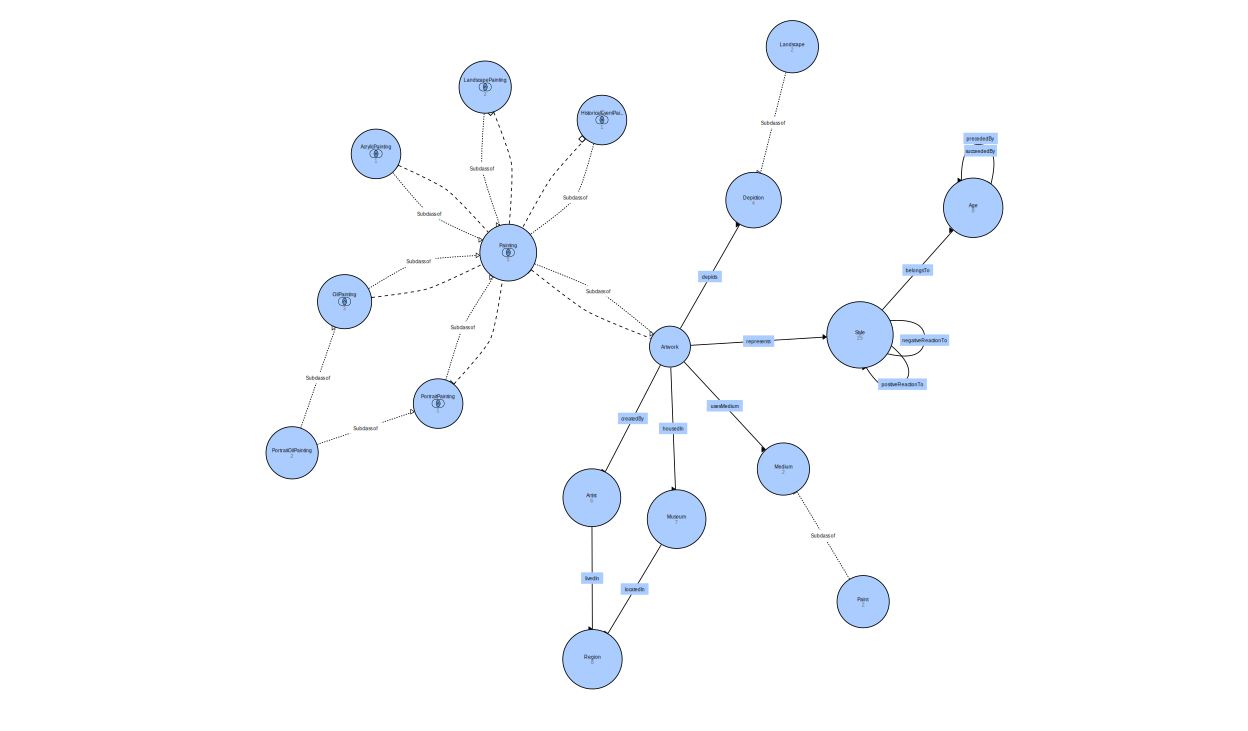
\includegraphics[width=\linewidth]{images/onto.png}  
  \caption{Визуализация на онтологията в WebVOWL}
\end{figure}

\section{Изводи}
\subsection{Изводи от вида $KB \vDash (d \sqsubseteq e)$}
Ще докажем, че $\text{PortraitOilPainting} \sqsubseteq \text{Artwork}$:
\begin{align*}
  \text{PortraitOilPainting} 
  \doteq & \text{[AND PortraitPainting OilPainting]} \\
  \doteq & \text{[AND} \\
          & \quad \text{[AND Painting [FILLS :depicts Portrait]]} \\
          & \quad \text{[AND Painting [FILLS :usesMedium OilPaint]]]} \\
  \doteq & \text{[AND} \\
          & \quad \text{Painting} \\
          & \quad \text{[FILLS :depicts Portrait]} \\
          & \quad \text{[FILLS :usesMedium OilPaint]]} \\
  \doteq & \text{[AND} \\
          & \quad \text{[AND Artwork} \\
          & \qquad \text{[EXISTS 1 :depicts]} \\
          & \qquad \text{[EXISTS 1 :hasMedium]]} \\
          & \quad \text{[FILLS :depicts Portrait]} \\
          & \quad \text{[FILLS :usesMedium OilPaint]]} \\
  \doteq & \text{[AND Artwork} \\
          & \quad \text{[EXISTS 1 :depicts]} \\
          & \quad \text{[EXISTS 1 :usesMedium]} \\
          & \quad \text{[FILLS :depicts Portrait]} \\
          & \quad \text{[FILLS :usesMedium OilPaint]]} \\
  \doteq & \text{[AND Artwork} \\
          & \quad \text{[FILLS :depicts Portrait]} \\
          & \quad \text{[FILLS :usesMedium OilPaint]]} \\
  \sqsubseteq & \text{Artwork}
\end{align*}

\subsection{Изводи от вида $KB \vDash (c \rightarrow e)$}
Ще докажем, че $\text{GirlWithAPearlEarring} \rightarrow \text{PortraitOilPainting}$:
\begin{align*}
  \text{GirlWithAPearlEarring} 
  \rightarrow & \text{[AND}\\
              & \quad \text{\textcolor{blue}{Artwork}} \\
              & \quad \text{\textcolor{blue}{[FILLS :depicts Portrait]}} \\
              & \quad \text{[FILLS :createdBy JohannesVermeer]} \\
              & \quad \text{\textcolor{blue}{[FILLS :usesMedium OilPaint]}} \\
              & \quad \text{[FILLS :represents Baroque]} \\
              & \quad \text{[FILLS :housedIn Mauritshuis]]} \\
\end{align*}


\begin{align*}
  \text{PortraitOilPainting}\doteq & \text{[AND}\\
  & \quad \text{\textcolor{blue}{Artwork}} \\
  & \quad \text{\textcolor{blue}{[FILLS :depicts Portrait]}} \\
  & \quad \text{\textcolor{blue}{[FILLS :usesMedium OilPaint]}]} \\
\end{align*}
\subsection{Класификация}
Ще въведем концепта $\text{HistoricalEventPainting}\doteq \text{[AND Painting [FILLS :depicts HistoricalEvent]]}$, за който очакваме:
\begin{align*}
  \text{Painting} \sqsubseteq \text{HistoricalEventPainting} \sqsubseteq \text{HistoricalEventOilPainting}
\end{align*}
В действителност, 
\begin{align*}
  S =& \left\{\text{Painting}\right\}\\
  G =& \left\{\text{HistoricalEventOilPainting}\right\}
\end{align*}
Окончателно:
\begin{figure}[H]
    \centering
    \begin{minipage}{0.45\textwidth}
        \centering
        \begin{tikzpicture}
            \node (Thing) at (0,0) {Thing};
            \node (Artwork) at (0,-1.5) {Artwork};
            \node (Painting) at (0,-3) {Painting};
            \node (OilPainting) at (-2,-4.5) {OilPainting};
            \node (HistoricalEventOilPainting) at (-1,-6) {HistoricalEventOilPainting};
            \node (Ellipsis) at (2,-4.5) { ... };

            \draw[->] (Thing) -- (Artwork);
            \draw[->] (Artwork) -- (Painting);
            \draw[->] (Painting) -- (OilPainting);
            \draw[->] (Painting) -- (HistoricalEventOilPainting);
            \draw[->] (Painting) -- (Ellipsis);
        \end{tikzpicture}
    \end{minipage}%
    \hspace{1cm} % Add space between diagrams
    \begin{minipage}{0.45\textwidth}
        \centering
        \begin{tikzpicture}
            \node (Thing) at (0,0) {Thing};
            \node (Artwork) at (0,-1.5) {Artwork};
            \node (Painting) at (0,-3) {Painting};
            \node (OilPainting) at (-3,-4) {OilPainting};
            \node (HistoricalEventPainting) at (0,-4.5) {\textcolor{red}{HistoricalEventPainting}};
            \node (HistoricalEventOilPainting) at (-1,-6) {HistoricalEventOilPainting};
            \node (Ellipsis) at (3,-4) { ... };

            \draw[->] (Thing) -- (Artwork);
            \draw[->] (Artwork) -- (Painting);
            \draw[->] (Painting) -- (OilPainting);
            \draw[->] (Painting) -- (HistoricalEventPainting);
            \draw[->] (Painting) -- (Ellipsis);
            \draw[->] (HistoricalEventPainting) -- (HistoricalEventOilPainting);
            \draw[->] (OilPainting) -- (HistoricalEventOilPainting);  % Missing connection added here
        \end{tikzpicture}
    \end{minipage}
    \caption{Класификация на новия концепт \emph{HistoricalEventPainting}}
\end{figure}
\pagebreak

\section{Заявки към БД}
Примерните заявки по-долу могат да бъдат изразени чрез разширение на езика $\mathcal{DL}$, което поддържа променливи и отрицания\cite{halReasoningDescription}.
\begin{itemize}
  \item Да се намери всяка картина, която е изложени в музей, разположен  в регион, различен от този, където е живял художникът ѝ
    \begin{align*}
      \text{MovedPainting} \doteq
      &\text{[AND}\\
      &\quad\text{[FILLS :createdBy [AND Artist [FILLS :livedIn ?artistRegion]]]}\\
      &\quad\text{[FILLS :housedIn [AND Museum [NOT [FILLS :locatedIn ?artistRegion]]]]]}
    \end{align*}
  \item Да се намерят тези художници, които са изработили портрети с различни графични средства:
  \begin{align*}
    \text{PortraitMaster ?artist} \doteq \\
    &\text{[AND} \\
    &\quad \text{Artist} \\
    &\quad \text{[EXISTS 1} \\
    &\quad \quad \text{[AND PortraitPainting} \\
    &\quad \quad \quad \text{[FILLS :usesMedium ?medium1]} \\
    &\quad \quad \quad \text{[FILLS :createdBy ?artist]]]} \\
    &\quad \text{[EXISTS 1} \\
    &\quad \quad \text{[AND PortraitPainting} \\
    &\quad \quad \quad \text{[FILLS :usesMedium ?medium2]} \\
    &\quad \quad \quad \text{[FILLS :createdBy ?artist]]]}\\
    &\quad \text{[NOT [?medium1 = ?medium2]]]}
  \end{align*}
\end{itemize}
\pagebreak
Синтаксисът на Protege не позволява променливи, но заявките могат да бъдат изразени чрез SPARQL по следния начин:
\begin{lstlisting}[language=SPARQL]
  PREFIX rdf: <http://www.w3.org/1999/02/22-rdf-syntax-ns#>
  PREFIX owl: <http://www.w3.org/2002/07/owl#>
  PREFIX rdfs: <http://www.w3.org/2000/01/rdf-schema#>
  PREFIX xsd: <http://www.w3.org/2001/XMLSchema#>
  PREFIX : <http://example.org/art_ontology.owl#>

  SELECT DISTINCT ?painting
  WHERE {
    ?painting rdf:type/rdfs:subClassOf* :Painting .
    ?painting :createdBy ?artist .
    ?painting :housedIn ?museum .
    ?artist :livedIn ?artistRegion .
    ?museum :locatedIn ?museumRegion .
    FILTER (?artistRegion != ?museumRegion)
  }

  SELECT DISTINCT ?artist
  WHERE {
    ?painting1 :depicts :Portrait .
    ?painting1 :createdBy ?artist .
    ?painting1 :usesMedium ?medium .

    ?painting2 :depicts :Portrait .
    ?painting2 :createdBy ?artist .
    ?painting2 :usesMedium ?otherMedium .
    FILTER (?medium != ?otherMedium)
  }
\end{lstlisting}
\begin{figure}[H]
  \includegraphics[width=\linewidth]{images/q1.png}
  \par
  \vspace{1cm}
  \includegraphics[width=\linewidth]{images/q2.png}
  \caption{Резултати от изпълнението на \emph{SPARQL} заявките в \emph{Protege}}
\end{figure}
\pagebreak

\section{Сравнение с други онтологии. Силни и слаби страни}
Кратко търсене в интернет откри много ограничено множество онтологии на естествен език, които са посветени на изкуството, сред които най-популярна е тази на Oxford\cite{Davies2009-hf}. Опит за достъп на 14.12.2024 чрез университетския ми профил върна грешка. 
\newline
Търсенето обаче не откри онтологии, които са машинно четими. Затова ще посоча някои обективни предимства, недостатъци и възможности за подобрения, които не са базирани на съпоставка с други онтологии:
\begin{itemize}
  \item онтологията е консистентна
  \item зададени са подходящ брой ограничения над ролите, които да помогнат в логическите изводи, но да не намалят изразителната сила на онтологията - например ролята \emph{represents} не е функционална, което отразява възможността едно произведение на изкуството да е екземпляр на повече от един стил
  \item онтологията е проектирана да подлежи на лесно разширение:
  \begin{itemize}
    \item за различни видове техники - може да бъдат добавени концепти като \emph{Technique}
    \item за всякакви видове изкуство чрез общия концепт \emph{Artwork}, който може да бъде разширен не само с \emph{Painting}, но и други видове творби - например скулптури, чрез \emph{Sculpture} чрез допълнителни ограничения с други концепти, например \emph{Medium}, към който може да бъдат добавени константи или подконцепти като \emph{HardMaterial, Marble} и др.
  \end{itemize}
  \item могат да бъдат дефинирани роли, задаващи точни години за началото и края на епохите, които, с подходящи правила за извод, могат да заменят релациите \emph{precededBy} и \emph{succeededBy}. По този начин епохите могат да се застъпват. Тази онтология умишлено не беше проектирана така с цел да бъдат спазени изискванията за брой и вид на ролите.
  \item съществуват десетки други стилове и хиляди произведения на изкуството, които не фигурират в онтологията и могат да бъдат добавени след консултация с експерт в областта. 
\end{itemize}

\section{Използвани технологии}
Онтологията е реализирана и проверена за консистентност на \emph{Python} с библиотеката \emph{owlready2}. \emph{SPARQL} заявките са изпълнени с \emph{Protege}. За визуализацията е използван \emph{WebVOWL}.
\pagebreak

\nocite{wikipediaCampbellsSoup,wikipediaGirlWith,wikipediaMonaLisa,wikipediaPortraitChalk,wikipediaThird1808,wikipediaHaystacksMonet,wikipediaStarryNight,wikipediaPeriodsWestern,wikipediaVisualArts,studiobinderHistoryTimeline}
\printbibliography

\end{document}
